\documentclass[]{article}
\usepackage{amsmath,amsfonts,amssymb,fancyhdr, enumerate, graphicx}
\usepackage[bottom]{footmisc}
\usepackage{setspace}
\usepackage{cite}
\doublespacing
\graphicspath{ {/LaTeX Images} }

\pagestyle{fancy}  
\oddsidemargin 1cm
\hoffset-1cm
\voffset-0.5cm
\topmargin-1.4cm
\textheight 24cm \textwidth 16.5cm \parindent 0.5cm

\begin{document}

\title{Mathematical Models of Gene Regulation}
\author{N. Horowitz, D, Picone, S. Condylios, T. Dwyer and M.Pauly}
\date{Today}
\maketitle

\section*{Abstract}
This paper explores the dynamics of gene regulation and degradation. We first examine the self regulation of a single gene before moving to multi-gene systems and finally to moving to a more complex regulatory system. We examine how WOR1, WOR 2 and EFG regulate each other in \textit{Candida albicans} modelling the system using Matlab and investigative techniques.
\section*{Introduction}

\pagebreak
\section*{Methods}

We began by investigating a single gene self regulating itself in Matlab. Genes code for proteins through a chain of processes.  In the case of Candida Albicans WOR1 binds to it's own DNA regulatory region which in turn activates the production of more WOR1 creating a positive feed back loop. 

A Diagram for the system is given below:\\

\begin{center}
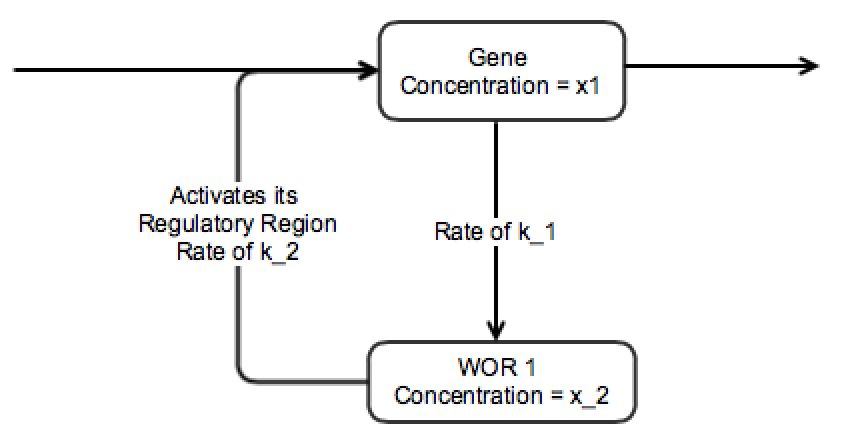
\includegraphics[scale = 0.75]{Posfeed.png}
\end{center}

The Rate of change for WOR1 is a system with an input of activation rate dependent upon the amount of $x_1$ and a output given by the degradation of itself $x_1$. The equation governing $x_1$ is a little more complex. As the activation can only occur on certain sites. The fraction of these occupied sites is given by Hill's equation \cite{Hill}. The system of equations is given below.

\begin{align}
\frac{dx_1}{dt} &= k_1\left(\frac{x_2^n}{\alpha^n + x_2^n}\right) - \gamma_1x_1\\
\frac{dx_2}{dt} &= k_2x_1 -\gamma_2x_2
\label{eq:posfeed}
\end{align}

	%insert image of equations here
Where:
\begin{itemize}
	\item $x_1 =$ mRNA concentration
	\item $x_2 =$ protein concentration
	\item $k(1), k(2) > 0$ production rate constants
	\item $\gamma(1), \gamma(2) > 0$ degradation rate constants
\end{itemize}


This system of equations was the analysed using Matlab and it's ode45 function. The first step in analysing this system was comparing the fraction of the occupied sites against the amount of WOR1. 

\begin{figure}[h]
\caption{Model of occupied reaction sites versus concentration of WOR1}
\centering
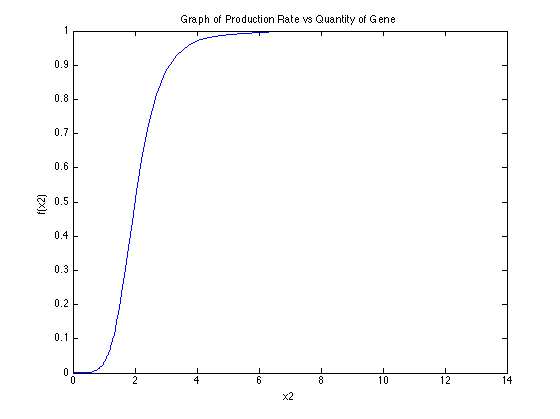
\includegraphics[scale = 0.5]{prodRateVsQuant.png}
\label{fig:Hill}
\end{figure}

We can see from Figure \ref{fig:Hill} that there are two distinct states,  a state of no occupation and a state of complete occupation. This does not, however describe how the system behaves around these two states. To gain more insight into the behaviour of this system we modelled the nullclines as described by 
	\begin{align}
		\dot{x}_1=0 \Rightarrow x_1=\frac{k_1}{\gamma_1}f(x_2)\\
		\dot{x}_2=0 \Rightarrow x_1=\frac{k_2}{\gamma_2}f(x_2)
	\end{align}

The Phase portraits around each stationary point were also modelled in Figure \ref{fig:phaseport}  to investigate the stability of each point.

\begin{figure}[h]
\caption{Nullclines for positive feedback system}
\centering
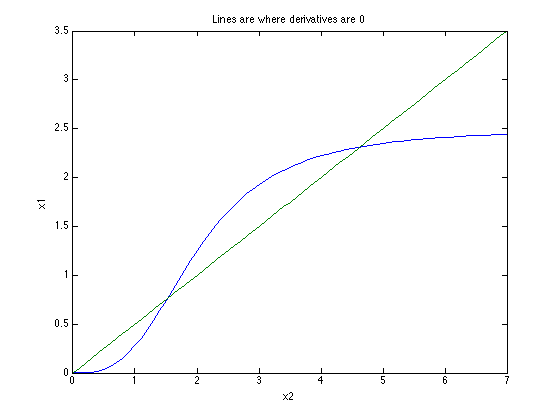
\includegraphics[scale = 0.5]{zeros.png}
\label{fig:nullclines}
\end{figure}

\pagebreak 


\begin{figure}[h]
\caption{Phase Portraits for the three stationary points}
\centering
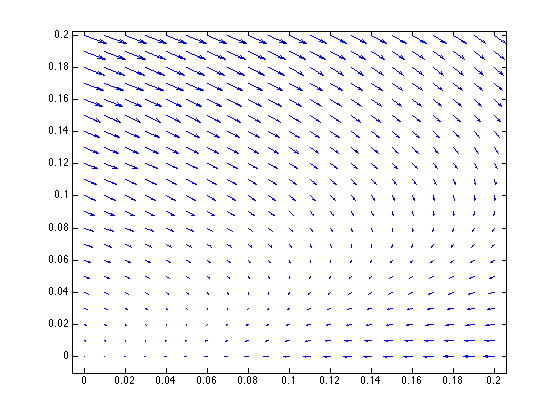
\includegraphics[width=.3\textwidth]{zerozero.png}\hfill
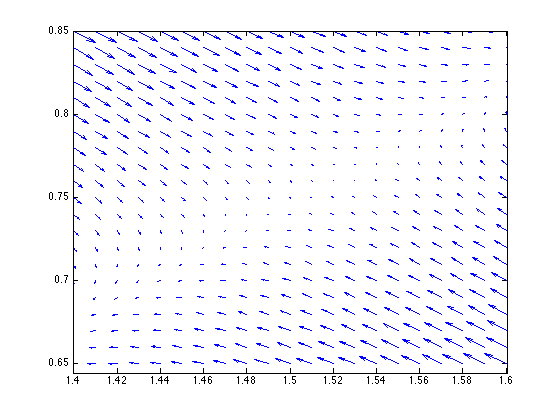
\includegraphics[width=.3\textwidth]{unstable.png}\hfill
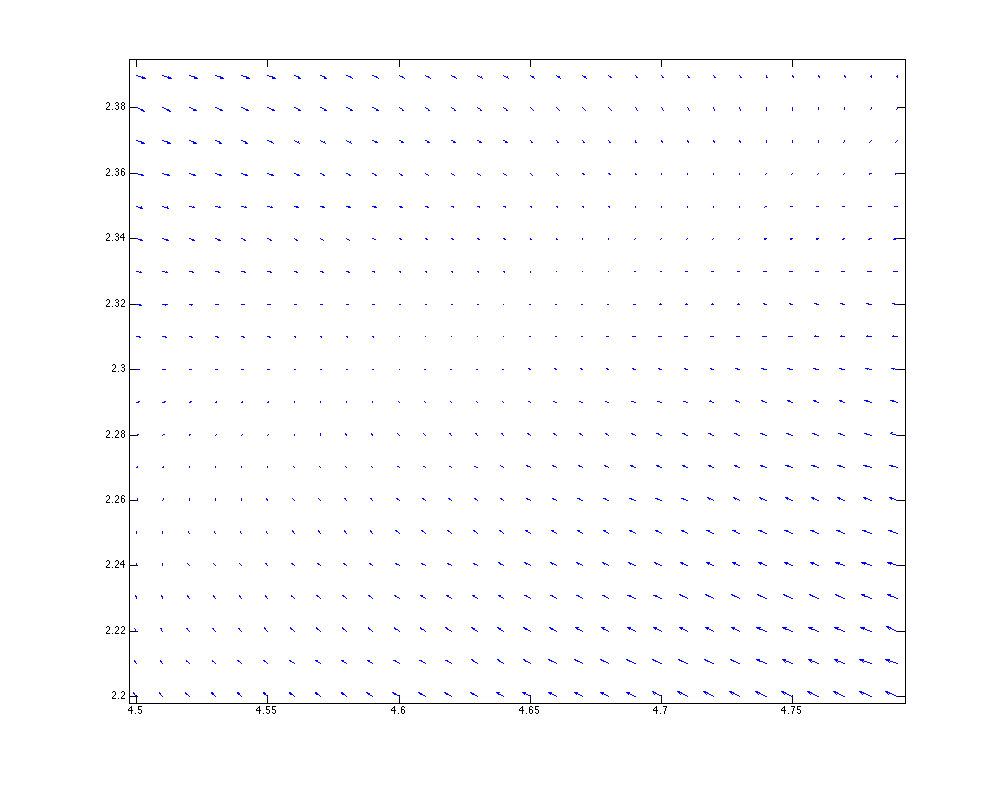
\includegraphics[width=.3\textwidth]{max.png}
\label{fig:phaseport}
\end{figure}

Figure \ref{fig:nullclines} suggests that there are three stationary points of which the rate of change for $x_1$ or $x_2$ is zero. Further investigation using Figure \ref{fig:phaseport} reveals that the first and last points are stable but the middle point is an unstable stationary point. Thus we can conclude that this system of equation is bistable. The stability points occur when all the reaction sites are occupied or when none of them are. This models very closely the observed opaque switching behaviour of the Candida Albans in the absence of an interim stability point.\\ 

 \pagebreak

\subsection{Negative feedback loop}
Gene's can also have negative feedback loops in them, where the production of a protein inhibits the production of itself. One such example of this is ????????????.

The previous equations for modelling positive feedback as described in Equation \pageref{eq:posfeed} can be modified to describe negative feedback in a gene. 

%% Finished %%

Using ode45 to solve this system we produced graphs showing the time development of the system showing the concentrations of proteins and mRNA. These graphs demonstrated interesting behaviours when given appropriate initial conditions and constants.

The system has one steady state at $\mathbf{\dot{x}}=0$, solving this we find:
	\begin{align}
		\dot{x}_1=0 \Rightarrow x_1=\frac{k_1}{\gamma_1}f(x_2)\\
		\dot{x}_2=0 \Rightarrow x_1=\frac{k_2}{\gamma_2}f(x_2)
	\end{align}
This state is stable and after perturbation the system will return to homeostasis.
\section*{Discussion}

\section*{Bibliography}

\bibliographystyle{unsrt}


\bibliography{Bibliography}
http://www-sop.inria.fr/comore/arcgdyn/28fev/arc03-intro.pdf
\end{document}